%v1
\documentclass{amsart}
\usepackage{amssymb, amsmath, amsfonts, amsthm}
\usepackage{graphics, enumerate, mathrsfs, mathtools,soul,csquotes}
\usepackage[color=red!40]{todonotes}
\usepackage{tikz-cd}
\usetikzlibrary{positioning,arrows,scopes}
%\usepackage{fancyhdr}
%\usepackage{geometry}
%\pagestyle{fancy}

% link highlighting
\definecolor{cadmiumgreen}{rgb}{0.0, 0.42, 0.24}
\usepackage[
colorlinks, citecolor=cadmiumgreen,
pagebackref,
pdfauthor={David Harry Richman}, 
pdfstartview ={FitV},
bookmarksdepth=3,
]{hyperref}
\hypersetup{
	pdftitle={Tutte power series on metric graphs},
}

\usepackage[
	backrefs,
	% msc-links,
	nobysame,
	lite,
	non-sorted-cites,
]{amsrefs} 

% COMMENT OUT FOR FINAL VERSION
\usepackage[inline]{showlabels}
\renewcommand{\showlabelfont}{\tiny\sffamily}

\newtheorem{thm}{Theorem}
\newtheorem*{thm*}{Theorem}
\newtheorem{obs}[thm]{Observation}
\newtheorem{prop}[thm]{Proposition}
\newtheorem{lem}[thm]{Lemma}
\newtheorem{cor}[thm]{Corollary}

\theoremstyle{definition}
\newtheorem{prob}[thm]{Problem}
\newtheorem{dfn}[thm]{Definition}
\newtheorem{eg}[thm]{Example}
\newtheorem{rmk}[thm]{Remark}
\newtheorem{conj}[thm]{Conjecture}
\newtheorem{fact}[thm]{Fact}

\newcommand{\CC}{\mathbb{C}}
\newcommand{\FF}{\mathbb{F}}
\newcommand{\RR}{\mathbb{R}}
\newcommand{\ZZ}{\mathbb{Z}}
\newcommand{\QQ}{\mathbb{Q}}
\newcommand{\NN}{\mathbb{N}}
\newcommand{\PP}{\mathbb{P}}
\newcommand{\cO}{\mathcal{O}}
\newcommand{\cU}{\mathcal{U}}
\newcommand{\cL}{\mathcal{L}}
\newcommand{\fg}{\mathfrak{g}}

\newcommand{\RRpos}{\RR_{>0}}
\newcommand{\RRnneg}{\RR_{\geq 0}}
\newcommand{\en}{n}

\DeclareMathOperator{\val}{val}
\DeclareMathOperator{\trop}{trop}
\DeclareMathOperator{\rspan}{row.span}
\DeclareMathOperator{\Sym}{Sym}
\DeclareMathOperator{\Div}{Div}
\DeclareMathOperator{\Eff}{Eff}
\DeclareMathOperator{\Supp}{Supp}
\DeclareMathOperator{\indeg}{indeg}
\DeclareMathOperator{\Pic}{Pic}
\DeclareMathOperator{\Jac}{Jac}
\DeclareMathOperator{\Mat}{Mat}
\DeclareMathOperator{\Arg}{Arg}
%\DeclareMathOperator{\ker}{ker}
\DeclareMathOperator{\coker}{coker}
\DeclareMathOperator{\Capacity}{\textsc{cap}}
\DeclareMathOperator{\coamoeba}{co\mathcal{A}}
\DeclareMathOperator{\PL}{PL}
%%% use either \Delta or Div %%%
\DeclareMathOperator{\Divisor}{\Delta}
\DeclareMathOperator{\zspan}{span}
\DeclareMathOperator{\im}{im}
\DeclareMathOperator{\red}{red}
\DeclareMathOperator{\Br}{Brk}
\DeclareMathOperator{\ev}{ev}
\DeclareMathOperator{\vol}{vol}
\DeclareMathOperator{\coeff}{coeff}

\renewcommand{\Re}{\mathrm{Re}}
\newcommand{\dsp}{\displaystyle}
\newcommand{\pderiv}[1]{\frac{\partial}{\partial{#1}}}
\newcommand{\angles}[1]{\langle {#1} \rangle}
% formal q-analog
\newcommand{\fanalog}[2]{[\![#2]\!]_{#1}}
\newcommand{\ufanalog}[1]{\fanalog{1 + u}{#1}}
% non-formal q-analog
\newcommand{\analog}[2]{[#2]_{#1}}
% moduli space of graphs
\newcommand{\Mgraphg}{\mathcal M_g^{\mathrm{graph}}}
\newcommand{\Mggraph}{\Mgraphg}

% for comments
\newcommand{\harry}[1]{{\color{red} \sf $\diamondsuit$ {#1} $\diamondsuit$ }}
\newcommand{\note}[1]{\harry{#1}}

\begin{document}
\title
[Tutte evaluations on metric graphs]
{Tutte evaluations on metric graphs and rank-generating power series}
%{Tutte power series and Tutte evaluations on the moduli space of metric graphs}
\author{David Harry Richman}
\date{v1, \today  \,(Preliminary draft, not for circulation).}
\thanks{This work was partially supported by NSF grant DMS-1600223
and a Rackham Predoctoral Fellowship.}


\begin{abstract}
We define a % formal power series 
Tutte power series for a metric graph with arbitrary positive real edge lengths, 
%called the Tutte power series,
% which is invariant under subdivision of edges.
which recovers the usual Tutte polynomial when all edge lengths are positive integers.
We prove that %for positive inputs, 
evaluation of the Tutte power series
defines a continuous function of the moduli space of metric graphs,
under certain constraints on the input parameters.
%which also extends to the compactification by tropical curves.
The evaluations give rise to a large family of functions generalizing the function that sends a metric graph to the volume of its graph Jacobian.
%We study how Tutte power series evaluations are
%related to various structures on a metric graph.
This is related to string theory.
\end{abstract}
\maketitle

\setcounter{tocdepth}{1}
\tableofcontents

\section{Introduction}
Given a graph $G$, the Tutte polynomial $T(G;x,y)$ is 
%an important graph invariant,
a two-variable polynomial %ssigned to graph $G$,
introduced by Tutte in \cite{Tut}.
Many important graph invariants arise as evaluations of 
the Tutte polynomial %$T(G; x,y)$ 
at specific integer parameters $x$, $y$.
One particular evaluation of the Tutte polynomial, $T(G; 1, 1)$ is the number of spanning trees of $G$.
In tropical geometry, it is well-known that the number of spanning trees on a graph has a ``continuous generalization'' as the volume of the Jacobian of a metric graph (a.k.a. an abstract tropical curve)~\cites{MZ,BF,ABKS}.
This motivates the question: can other Tutte polynomial evaluation be generalized to arbitrary metric graphs?
In this paper, we show that the function sending a graph $G$ to its Tutte polynomial evaluation $T(G; x, y)$ can be extended to a continuous invariant on the space of metric graphs, whenever $x > 0$.
This is achieved by defining a rank generating power series on a metric graph,
which generalizes the rank generating polynomial on a graph.

As a consequence, the Tutte evaluation at $(x, y)$ defines a continuous function on the space of metric graphs of fixed genus.
\begin{thm}
	For fixed real constants $x$ and $y$, let $\ev_{(x, y)}(G)$ denote the evaluation of the Tutte polynomial of $G$ at $(x, y)$.
	If $x > 0$, then $\ev_{(x, y)}: \Mgraphg \to \RR$ defines a continuous function on the space of metric graphs of genus $g$.
\end{thm}

For a comprehensive modern overview of the Tutte polynomial see \cites{BO, EMM}.

\subsection{Rank generating power series}
The following characterization of the Tutte polynomial was initially introduced by Crapo \cite{Cra}, 
using the  {\em rank generating function} of $G$
(see also \cite{EMM}*{Definition 3}).
Given a connected graph $G $, 
%we can define the Tutte polynomial of $G$ by 
the Tutte polynomial of $G$ is 
\begin{equation}
\label{eq:tutte-graph}
T(G; x,y) = \sum_{A \subset E(G)} (x-1)^{h_0(G\backslash A) - 1}(y-1)^{h_1(G\backslash A)}
\end{equation}
where $G\setminus A$ denotes the graph with edges in $A$ deleted,
and $h_0$ and $h_1$ denote the zeroth and first Betti numbers of 
a topological space.
In graph theoretic terms,
\begin{align*}
h_0(G) &= \#(\text{connected components of }G), \quad\text{and}\\
h_1(G) &= \# E(G) - \# V(G) + h_0(G) .
\end{align*}

The key insight of this paper is that this polynomial, associated to any graph, may be extended to a power series associated to any metric graph.
As a consequence, evaluation of the Tutte polynomial, at certain real parameters, extends to a continuous function on the moduli space of metric graphs.

\subsection{Statement of results}
Suppose $\Gamma$ is a metric graph with combinatorial model $\Gamma = (G,\ell)$,
where $\ell : E(G) \to \RRpos$ assigns a positive length to each edge of $G$.

%We can recover a power series expression for $T(\Gamma; x,y)$ by a simple change of variables.
We define the {\em Tutte power series}
$T^+(\Gamma; u,w)$ %$ := T(\Gamma; 1 + u, 1 + w) $
of $\Gamma$ as
\begin{equation}
\label{eq:tutte-power-series}
	T^+(\Gamma; u,w) = \sum_{A \subset E(G)} \left( \prod_{e_i \in A} \fanalog{1 + u}{\ell(e_i)} \right)
	u^{h_0(G\backslash A) - 1}w^{h_1(G\backslash A)} 
\end{equation}
where $\fanalog{1 + u}{\alpha}$ denotes the formal power series  
\begin{equation}\label{eq:f-analog}
	\fanalog{1 + u}{\alpha} \coloneq \alpha + \binom{\alpha}{2} u + \binom{\alpha}{3} u^2 + \cdots
	\quad \in \RR[[u]]
\end{equation}
and
$\binom{\alpha}{k}$ % \coloneq 
denotes the polynomial
$\displaystyle \frac1{k!}\alpha(\alpha - 1) \cdots (\alpha - k + 1)$.
If all edges in $\Gamma$ have unit length, i.e. $\ell(e) = 1$, then \eqref{eq:tutte-power-series} reduces to the Tutte polynomial by the substitution $T(G; x, y) = T^+(\Gamma; x - 1, y - 1)$.

Our first main result is that the expression \eqref{eq:tutte-power-series} does not depend on the chosen model $(G,\ell)$ for the metric graph $\Gamma$.
\begin{thm}[Tutte power series]
\label{thm:intro-tutte-series}
Given a metric graph $\Gamma = (G,\ell)$,
the expression $T^+(\Gamma; u,w)$
is a well-defined power series in
$\RR[\![u]\!][w]$;
in particular,
$T^+(\Gamma; u,w)$ does not depend on the choice of model $(G,\ell)$ for $\Gamma$.
\end{thm}

To prove this result, we show that $T^+(\Gamma; u, w)$ satisfies a familiar deletion-contraction identity.
\begin{thm}[Deletion-contraction relation]
\label{thm:intro-deletion-contraction}
Given a metric graph $\Gamma = (G,\ell)$ and an edge $e \in E(G)$,
which is not a loop,
the Tutte power series satisfies
\begin{equation}
	T^+(\Gamma; u,w) = \fanalog{1 + u}{\ell(e)} \, T^+(\Gamma \backslash e; u,w) + T^+(\Gamma / e; u,w).
\end{equation}
\end{thm}

\subsection{Evaluating Tutte power series}

Instead of considering a fixed metric graph $\Gamma$,
% and varying the parameters $u,w$,
we can 
%fix a choice of $(u,w)$ and 
vary $\Gamma$ over a natural moduli space of metric graphs.
As $\Gamma$ varies, the value of $T^+(\Gamma;u,w)$ also varies continuously under certain mild assumptions on the parameters $(u, w)$.

Let $\Mgraphg$ denote the moduli space of stable metric graphs of genus $g$.
\begin{thm}[Continuity of Tutte evaluation]
\label{thm:tutte-eval-moduli}
	Let $u$ and $w$ be fixed real numbers, with $u > -1$.
	The Tutte evaluation at $(u,w)$,
	%on the moduli space of metric graphs (of genus $g$),
	\[ \ev^+(u,w) : \Gamma \,\mapsto\, T^+(\Gamma; u,w) ,\]
	defines a continuous function  
	${\rm ev}^+(u,w) : \Mgraphg \to \RR$ on the moduli space of stable graphs.
	Namely, 
	\begin{enumerate}[(i)]
	\item 
	(Continuity on cells)
	for each stable combinatorial graph $G$,
	the Tutte evaluation 
	$\ev^+(u,w) $ 
	defines a continuous function
	\[
		\ev^+(u,w) : \RRpos^{E(G)} \to \RR,
	\]
	where a point in the positive orthant $\RRpos^{E(G)}$
	represents a choice of positive, real edge lengths in $G$.
	% $\ell : E(G) \to \RRpos$.
	
	\item 
	(Continuity between cells)
	% If $u > -1$, then 
	As the length of a non-loop edge $e \in E(G)$ approaches zero in the metric graph $\Gamma = (G,\ell)$
	while all other edge lengths are fixed, the value of 
	%the Tutte evaluation 
	$\ev^+(u,w)$
	at $(G, \ell)$ %$\Gamma $ 
	approaches the value of $\ev^+(u,w)$ at the contraction 
	$\Gamma / e$. % = (G / e, \ell \big|_{E\setminus e})$.
	\end{enumerate}
\end{thm}

Note the power series \eqref{eq:f-analog} converges for $|u| < 1$, and in this range satisfies
\[ 
	\fanalog{1}{\alpha} = \alpha
	\qquad\text{and}\qquad
	\fanalog{1 + u}{\alpha} = \frac{(1+u)^\alpha - 1}{u}
	%= \sum_{k \geq 1} \binom{\alpha}{k}u^{k-1} 
	\qquad \text{if } u \neq 0.
\]

\begin{eg}
[$u = 0$, $w = 0$]
%The Tutte evaluation $\ev^+(0, 0)$ 
%on a graph $G$ gives the number of spanning trees.
On a metric graph, the Tutte evaluation $\ev^+(0, 0)$ gives the volume of the Jacobian of
$\Gamma = (G,\ell)$,
which can be expressed as a weighted sum of spanning trees of $G$\todo{[cite a reference]}.
The function $\ev^+(0, 0)$ is continuous on $\Mgraphg$, 
and extends continuously to $\overline{\Mgraphg}$ 
(where it has value zero on the boundary).
\end{eg}
\begin{eg}
[$u = -1$, $w = 1$]
The Tutte evaluation $\ev^+(-1, 1)$ 
on $\Gamma = (G,\ell)$ gives the number of totally cyclic orientations of $\Gamma$.
This number does not depend on the edge lengths of $\Gamma$;
i.e. $\ev^+(-1, 1)$
 is constant on metric graphs %$\Gamma = (G,\ell)$ 
of a fixed combinatorial model $G$.
However, $\ev^+(-1, 1)$ is not continuous as some edge length approaches $0$.
Namely, the value of $T(G; -1, 1)$ generally differs from the value of $T(G/e; -1, 1)$
after contracting an edge.

For example, the number of totally cyclic orientations of graphs of genus two are shown below.

\begin{figure}[h]
\begin{tabular}{ccc}
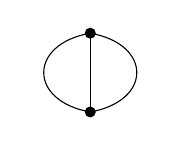
\begin{tikzpicture}
	\draw (0,0) -- (0,1);
	\draw (0,0) to[bend left=80,min distance=8mm] (0,1);
	\draw (0,0) to[bend right=80,min distance=8mm] (0,1);
	\fill (0,0) circle[radius=0.7mm];
	\fill (0,1) circle[radius=2pt];
\end{tikzpicture}
&
\begin{tikzpicture}[every loop/.style={min distance=15mm}]
	\draw (0,0) to[out=140,in=220,loop] (0,0);
	\draw (0,0) to[in=-40,out=40,loop] (0,0);
	\fill (0,0) circle[radius=2pt];
\end{tikzpicture}
&
\begin{tikzpicture}
	[every loop/.style={min distance=15mm}]
	\draw (0,0) to[out=140,in=220,loop] (0,0);
	\draw (0,0) -- (1,0);
	\draw (1,0) to[out=-40,in=40,loop] (1,0);
	\fill (0,0) circle[radius=2pt];
	\fill (1,0) circle[radius=2pt];
\end{tikzpicture}
\\
$6$ & $4$ & $0$
\end{tabular}
\caption{Number of totally cyclic orientations.}
\end{figure}
\end{eg}

\subsection{Previous work} 

The multivariate Tutte polynomial \cite{Sok-potts}
is also known as the {\em Potts-model partition function}.
Sokal \cite{Sok-potts} asks:
\begin{displayquote}
	Let me conclude by observing that numerous specific evaluations of the Tutte polynomial have been given combinatorial interpretations, 
	as counting some set of objects associated to the graphs $G$. 
	It would be an interesting project to seek to extend these counting problems to ``counting with weights,''
	i.e., to obtain suitably defined univariate or multivariate generating polynomials for the objects in question as specializations of 
	$Z_G(q,v)$ or $Z_G(q,\mathbf{v})$, respectively.
\end{displayquote}
\todo[inline]{Is the ``continuous'' version of $Z_g(q, v)$ described? if so, link it}

Several authors have investigated the behavior of the Tutte polynomial under the operation of subdividing an edge into multiple edges.

Previous work on {\em chain polynomials}:

The identities presented in this paper are essentially in the work of Read and Whitehead~\cite{RW2}, but with the restriction that edge lengths are positive integers. In their work, edge lengths are called ``chain lengths.''

The family of graphs obtained by varying chain lengths of a fixed graph is called a ``homeomorphism class'' of graphs.

Read and Whitehead \cite{RW2}
\cites{RW1,RW2}

The essential contribution of this work is to enforce a dependence of the edge weights $(\alpha(e))$ on the polynomial parameter $u$, namely $\alpha(e) = \fanalog{1 + u}{\ell(e)}$.

Traldi~\cite{Tra1} considers the weighted Tutte polynomial
\[
	\widetilde T^+(G; u,w) = \sum_{A \subset E} \left( \prod_{e \in A} c(e) \right) u^{h_0(G|A)} w^{h_1(G|A)} .
\]
The same weighted polynomial was previously studied by Fortuin--Kasteleyn~\cite{FK}, but in harder-to-understand notation for a modern reader.


Brylawski \cite{Bry}

Traldi \cites{Tra1,Tra2,Tra3}

Application: Zeros of Tutte polynomials?

Jackson and Sokal \cite{JS} study zero-free regions of the Tutte polynomial.

Ok and Perrett \cite{OP} study the density of the real zeros of the Tutte polynomial.


\subsection{Notation}

$\Gamma$ a compact metric graph

$G$ a finite graph, 
loops and parallel edges allowed,
possibly disconnected

$E(G)$ edge set of $G$

$V(G)$ vertex set of $G$

$(G,\ell)$ a combinatorial model for a metric graph,
where 
%$G$ is a combinatorial graph and 

$\ell : E(G) \to \RRpos$
is a length function on edges of $G$

$T(G; x,y)$ the Tutte polynomial of $G$

$T^+(G; u,w) = T(G; 1+u,1+w)$ ``additive'' centered Tutte polynomial

$T^+(\Gamma; u,w)$ the Tutte power series of $\Gamma$

% $D_N$ a divisor of degree $N$


% $\mu = \mu_\Gamma$ the canonical measure on a metric graph $\Gamma$

% \section{Background}

\section{\texorpdfstring{$q$}{q}-analogs}

For a positive integer $\en$, the {\em $q$-analog} $[\en]_q$ is defined as
the polynomial
\begin{equation*}
	[\en]_q = \frac{q^\en - 1}{q - 1}
	%= \frac{1 - q^\en }{1 - q} 
	= 1 + q + q^2 + \cdots + q^{\en -1} 
	\in \ZZ[q].
\end{equation*}
%When $\en$ is not a positive integer, the above expression is no longer a polynomial.
When $\en$ is not an integer, 
%the above expression is not even has 
$[\en]_q$ does not admit a Laurent expansion in the variable $q$.
However, we can obtain a well-defined power series under a simple change of variable.
Namely, note that
\[ 
	[\en]_{1+u} = \frac{(1+u)^\en - 1}{u}
= \sum_{k \geq 0} \binom{\en}{k+1}u^{k},
\]
and the binomial coefficient $\binom{n}{k}$ has a well-defined extension
\begin{equation}
\binom{\alpha}{k} = \frac{\alpha (\alpha-1) \cdots (\alpha-k+1)}{k!} 
\end{equation}
where $\alpha$ can be any real number.
% and $\binom{\alpha}{k}$ is the real number

by the binomial series expansion, so we have 
\begin{equation}
\fanalog{1+u}{\alpha} \coloneq \alpha + \binom{\alpha}{2} u + \binom{\alpha}{3} u^2 + \cdots
\in \RR[[u]] .
\end{equation}

\todo{
TODO: decide on notation
$\fanalog{q}{\alpha}$
$\analog{q}{\alpha}$
$[\![\alpha]\!]_q$
$\left[\alpha\right]_q$
}

\begin{fact}
\hfill
\begin{enumerate}
\item 
For a positive integer $n$, the expression $\analog{q}{n}$ is a polynomial in $\ZZ[q]$. 
As $q \to 1$, we have $\analog{q}{n} \to n$.
As $q \to 0$, we have $\analog{q}{n} \to 1$.

\item 
For a real number $\alpha$, the expression $\fanalog{1 + u}{\alpha}$ is a power series in $\RR[[u]]$.
As $u \to 0$, we have $\fanalog{1 + u}{\alpha} \to \alpha$.
\todo[inline]{If $\alpha$ is positive, then as $u \to -1$, we have $\fanalog{1 + u}{\alpha} \to 1$.}
\end{enumerate}
\end{fact}

For positive integers $n,m$ we have
\begin{equation*}
\analog{q}{n + m}
%=  [n ]_q + q^{n} [m]_q
 = \analog{q}{n} + \analog{q}{m} + (q-1) \analog{q}{n} \analog{q}{m} .
%[a + b]_q = [a]_q + q^a [b]_q = [a]_q + [b]_q + (q-1) [a]_q [b]_q .
\end{equation*}
The analogous identity holds for power series $\fanalog{1 + u}{\alpha}$.
\begin{prop}\label{prop:fanalog-add}
	For real numbers $\alpha,\beta$, we have
	\begin{align*}
	\fanalog{1 + u}{\alpha + \beta} 
	%&=  [\alpha]_{1+u} + (1+u)^{\alpha} [\beta]_{1+u} \\
	 &= \fanalog{1 + u}{\alpha} + \fanalog{1 + u}{\beta} + u \, \fanalog{1 + u}{\alpha} \fanalog{1 + u}{\beta} .
	\end{align*}
	as elements of $\RR[\![u]\!]$.
\end{prop}
\begin{proof}
First, observe that on the open disc $|u| < 1$, we have
\[
	1 + u \ufanalog{\alpha} = (1 + u)^\alpha,
\]
due to the binomial series identity.
Thus
\begin{align*}
	1 + u \ufanalog{\alpha + \beta} &= (1 + u)^{\alpha + \beta} 
	= (1 + u)^\alpha (1 + u)^\beta \\
	&= (1 + u \ufanalog{\alpha}) (1 + u \ufanalog{\beta}) \\
	&= 1 + u(\ufanalog{\alpha} + \ufanalog{\beta}) + u^2 \ufanalog{\alpha} \ufanalog{\beta},
\end{align*}
which implies the desired result.
\end{proof}



\section{Metric graphs}

A metric graph is a compact, connected metric space which comes from 
assigning edge lengths to a finite, connected graph.
If the metric graph $\Gamma$ comes from a combinatorial graph $G$ by 
assigning edge lengths $\ell : E(G) \to \RRpos$,
we say $(G,\ell)$ is a {\em combinatorial model} for $\Gamma$
and we write $\Gamma = (G,\ell)$.
%(A single metric graph generally has many different combinatorial models.)

\subsection{Graph terminology}
\begin{align*}
h_0(G| A) - 1 &= rk(G) - rk(A), \quad\text{and}\\
h_1(G| A) &= \#(A) - rk(A) .
\end{align*}


\subsection{Tutte polynomial}

\subsection{Deletion and contraction}

Suppose $\Gamma = (G,\ell)$, and $e \in E(G)$ is a non-loop edge.

The {\em edge deletion} $\Gamma \setminus e$ is the metric graph obtained from $\Gamma$ by removing the points in the interior of $e$.
The {\em edge contraction} $\Gamma / e$ is the metric graph obtained from $\Gamma$ by removing the points in the interior of $e$, and then joining the endpoints of $e$.

% [show a figure with examples]

\section{Tutte power series}

Let $T^+(\Gamma; u,w)$ be the power series in $\RR[\![u]\!][w]$
defined by
\begin{equation}
%\label{eq:tutte-power-series}
	T^+(\Gamma; u,w) = \sum_{A \subset E(G)} \left( \prod_{e \in A} \fanalog{1 + u}{\ell(e)} \right)
	u^{h_0(G\backslash A) - 1}w^{h_1(G\backslash A)} .
\end{equation}


\begin{prop}
\hfill
\begin{enumerate}
\item 
Let $\Gamma = \Gamma_1 \vee \Gamma_2$ denote the wedge sum of two metric graphs. Then
\[
	T^+(\Gamma_1 \vee \Gamma_2; u,w) = T^+(\Gamma_1; u,w) \, T^+(\Gamma_2; u, w).
\]

\item 
Let $\Gamma = \Gamma_1 \bigsqcup \Gamma_2$ denote the (disconnected) disjoint union of two metric graphs. Then
\[
	T^+(\Gamma_1 \sqcup \Gamma_2; u,w) = u\, T^+(\Gamma; u,w) \, T^+(\Gamma; u, w).
\]

\end{enumerate}
\end{prop}


\subsection{Deletion-contraction}

The Tutte polynomial $T(G; x,y)$ can be characterized inductively by the deletion-contraction relation:
\begin{equation*}
	T(G;x,y) = T(G \backslash e; x,y) + T(G / e; x,y).
\end{equation*}
if $e$ is not a loop or bridge,
along with the base cases 
\begin{equation*}
	T(G; x,y) = x^i y^j \qquad\text{if $G$ consists of $i$ bridges and $j$ loops.}
\end{equation*}
%for a loop edge and bridge edge.
%\begin{equation*}
%T(G;x,y) = \begin{cases}
%x & \text{if $G$ is a bridge} \\
%y & \text{if $G$ is a loop}.
%\end{cases}
%\end{equation*}

The Tutte power series $T^+(\Gamma; u,w)$ satisfies a similar deletion-contraction relation.

\begin{thm}\label{thm:deletion-contraction}
For a metric graph $\Gamma$,
\begin{equation}
	T^+(\Gamma; u,w) 
	= \fanalog{1 + u}{\ell(e)} T^+(\Gamma \backslash e; u,w) + T^+(\Gamma / e; u,w) .
\end{equation}
\end{thm}

\begin{proof}
Observe that
\[
	T^+(\Gamma; u,w) 
	= \sum_{A \subset E} (\cdots)
	= \sum_{\substack{A \subset E \\ e_0 \in A}} (\cdots) + \sum_{\substack{A \subset E \\ e_0 \not \in A}} (\cdots).
\]
The first sum reduces to
\begin{align*}
	&\sum_{\substack{A \subset E \\ e_0 \in A}} \left( \prod_{e \in A} \fanalog{1+u}{\ell(e)} \right) u^{h_0(G\setminus A)-1}w^{h_1(G\setminus A)}\\
	&\qquad\qquad = \fanalog{1+u}{\ell(e_0)} \sum_{\substack{A' \subset E \setminus e_0}} \left( \prod_{e \in A'}\fanalog{1+u}{\ell(e)} \right) u^{h_0(G\setminus e_0\setminus A)-1}w^{h_1(G\setminus e_0\setminus A)} \\[1.5em]
	&\qquad\qquad = \fanalog{1+u}{\ell(e_0)}\, T^+(G\setminus e_0;u,w),
\end{align*}
while the second sum reduces to
\begin{align*}
	&\sum_{\substack{A \subset E \\ e_0 \not\in A}} \left( \prod_{e \in A} \fanalog{1+u}{\ell(e)} \right) u^{h_0(G\setminus A)-1}w^{h_1(G\setminus A)}\\
	&\qquad\qquad = \sum_{\substack{A \subset E \setminus e_0}} \left( \prod_{e \in A} \fanalog{1+u}{\ell(e)} \right) u^{h_0(G \setminus A / e_0)-1}w^{h_1(G\setminus A / e_0)} \\[1.5em]
	&\qquad\qquad = T^+(G/ e_0;u,w).
\end{align*}
In the second equality, we use the fact that the quotient map $(G\setminus A) \to (G\setminus A)/e_0$ is a homotopy equivalence, so it preserves homology groups. The third line uses the fact that deletion and contraction commute, $(G \setminus A) / e_0 = (G / e_0) \setminus A$.
\end{proof}

\begin{eg}[Rank power series of a line]
Suppose $\Gamma$ is a segment of length $\alpha$,
then
%\[
%	T^+(\Gamma;u,w) 
%	= 1 + \fanalog{1 + u}{\alpha} u
%	= (1+u)^\alpha,
%\]
%which has power series expansion
\[
	T^+(\Gamma;u,w) 
% = \sum_{k=0}^\infty \binom{\alpha}{k} u^k
= 1 + \alpha u + \binom{\alpha}{2}u^2 + \cdots .
\]

If $G$ is a line graph consisting of $n$ edges,
then
\[
	%T(G;x,y) = x^n 
	%\qquad\text{and}\qquad 
	T^+(G;u,w) = (1+u)^n = 1 + nu + \binom{n}{2}u^2 + \cdots + u^n.
\]
\end{eg}

\begin{eg}[Rank power series of a circle]
If $\Gamma$ is a circle of length $\alpha$, then 
%\[
%	T^+(\Gamma;u,w) = w + \fanalog{1 + u}{\alpha} = w + \frac{(1 + u)^\alpha - 1}{u}
%\]
%which has power series expansion
\[
	T^+(\Gamma;u,w) = w + \alpha + \binom{\alpha}{2} u + \binom{\alpha}{3} u^2 + \cdots .
\]

Suppose $G$ is a cycle graph consisting of $n$ edges.
Then
%$$
%T(G;x,y) = x + x^2 + \cdots + x^{n-2} + x^{n-1} + y 
%= \frac{x^n - 1}{x - 1} + y - 1.
%$$
%and
$$
T^+(G;u,w) = n + \binom{n}{2}u + \binom{n}{3} u^2 + \cdots + nu^{n-2} + u^{n-1} + w
= \frac{(1+u)^n-1}{u} + w
$$
\end{eg}

\begin{eg}[Tutte power series of theta graph]
Suppose $G$ is the graph with two vertices connected by three edges.
Suppose $\Gamma$ is the metric graph which assigns lengths $a,b,c$ to the edges of $G$.
Then
\begin{multline*}
T^+(G;u,w) = ( \fanalog{1 + u}{a} \fanalog{1 + u}{b} + \fanalog{1 + u}{a} \fanalog{1 + u}{c} + \fanalog{1 + u}{b} \fanalog{1 + u}{c} ) \\
+ ( \fanalog{1 + u}{a} \fanalog{1 + u}{b} \fanalog{1 + u}{c} ) u 
+ (\fanalog{1 + u}{a} + \fanalog{1 + u}{b} + \fanalog{1 + u}{c}) w + w^2 .
\end{multline*}

%Using deletion-contraction, we also deduce
%\begin{align*}
%T^+(G;u,w) &= \fanalog{1 + u}{a} T^+(\text{circle of length }b+c) \\
%&\qquad\quad + T^+(\text{circle of length }b)T^+(\text{circle of length }c) \\
%&= \fanalog{1 + u}{a} ([b+c]_{1+u} + w)
%+ (\fanalog{1 + u}{b} + w) (\fanalog{1 + u}{c} + w) \\
%&= (\fanalog{1 + u}{a} [b+c]_{1+u} + \fanalog{1 + u}{b}\fanalog{1 + u}{c} ) + 
%(\fanalog{1 + u}{a} + \fanalog{1 + u}{b} + \fanalog{1 + u}{c}) w + w^2 .
%\end{align*}
\end{eg}

%\begin{align*}
%T^+(\Gamma;u,w) &= \fanalog{1 + u}{a}T^+() + T^+() \\
%&= \fanalog{1 + u}{a} [d]_{1+u} T^+(\text{circle of length }b+c+e+f) \\
%&\qquad\quad + \fanalog{1 + u}{a} T^+(\text{circle of length }b+c) T^+(\text{circle of length }e+f) \\
%&\qquad\quad + [d]_{1+u} T^+(\text{circle of length }b+f)T^+(\text{circle of length }c+e) \\
%&\qquad\quad + T^+(\text{banana of lengths }b,c,e,f) \\
%&= \sum_{k \geq 0} \binom{a}{k+1}u^k \sum_{k\geq 0} \binom{d}{k+1}u^k \left( \sum_{k\geq 0} \binom{b + c + e + f}{k+1} u^k + w\right) \\
%&\qquad\quad + \sum_{k \geq 0} \binom{a}{k+1}u^k \left( \sum_{k\geq 0} \binom{b+c}{k+1}u^k + w\right) \left(\sum_{k\geq 0} \binom{e+f}{k+1}u^k + w\right) \\
%&\qquad\quad + \sum_{k\geq 0}\binom{d}{k+1}u^k \left(\sum_{k\geq 0} \binom{b+f}{k+1}u^k + w \right) \left(\sum_{k\geq 0}\binom{c+e}{k+1}u^k + w\right) \\
%&\qquad\quad + \\
%&= \cdots \\
%\end{align*}

\subsection{Deleting bridges and contracting loops}
In this section we describe how the definition of Tutte power series $T^+(\Gamma;u,w)$
may be extended to a more general concept of metric graphs.

\begin{dfn}
A {\em genus-weighted metric graph}
$\Gamma = (G,\ell, \fg)$
consists of a graph $G = (V,E)$,
a length function $\ell : E \to \RRpos$ on edges,
and a genus function
$\fg: V \to \ZZ_{\geq 0}$ on vertices.
\end{dfn}

\begin{itemize}
\item
If $\Gamma = \bigcup_{i=1}^k \Gamma_i$ is a disjoint union of $k$ connected metric graphs $\Gamma_i$,
then 
\begin{align*}
T^+\left(\bigcup_{i=1}^k \Gamma_i ; u,w \right) 
&= u^{k-1}\, T^+\left(\vee_{i=1}^k \Gamma_i; u,w \right) .
% &= u^{k-1}\, \prod_{i=1}^k T^+(\Gamma_i; u,w )  .
\end{align*}

\item
If $\Gamma^{\fg} = (G,\ell,\fg)$ is a genus-weighted metric graph,
with underlying metric graph $\Gamma^0 = (G,\ell)$,
then
\[
	T^+(\Gamma^{\fg}; u,w) = w^{\sum \fg(v)} \, T^+(\Gamma^0; u,w).
\]
\end{itemize}

\subsection{Proofs}

\begin{proof}[Proof of Theorem~\ref{thm:intro-tutte-series}]
It sufficies to show that the Tutte power series is invariant 
under an edge subdivision.
Suppose $G = (V,E)$ contains the edge $e_0$, which we subdivide into $e_1 \cup e_2$ to obtain the graph $G'$.
Suppose $e_1$ has length $a$ and $e_2$ has length $b$, so that $e_0$ has length $a + b$.

By the deletion-contraction relation, Theorem~\ref{thm:deletion-contraction},
we have
\[
	T^+(G; u,w) = \fanalog{1 + u}{a + b} T^+(G\setminus e_0; u,w) + T^+(G/e_0; u,w)
\]
and 
\begin{align*}
	T^+(G'; u,w) &= \fanalog{1 + u}{a} T^+(G\setminus e_1; u,w) + T^+(G/e_1; u,w)\\
	&= \fanalog{1 + u}{a}\left(\fanalog{1 + u}{b} T^+(G\setminus\{e_1,e_2\}; u,w) + T^+(G \setminus e_1 / e_2; u,w)\right) \\
	&\qquad + \left(\fanalog{1 + u}{b} T^+(G/e_1 \setminus e_2; u,w) + T^+(G/\{e_1,e_2\}; u,w) \right)
\end{align*}
The compound contraction $G' / \{e_1, e_2\}$ is the same metric graph as $G / e_0$,
while the compound deletion $G' \setminus \{e_1, e_2\}$ is the disjoint union of an isolated vertex and the metric graph $G \setminus e_0$.
For the mixed deletion-contraction operations, 
\[
	G' \setminus e_1 / e_2 \cong G' / e_1 \setminus e_2 \cong G \setminus e_0.
\]

Therefore, 
\[
	T^+(G'; u,w) = (\fanalog{1 + u}{a} + \fanalog{1 + u}{b} + u\fanalog{1 + u}{a}\fanalog{1 + u}{b}) T^+(G\setminus e_0; u,w) + T^+(G/e_0; u,w) .
\]
and from here it suffices to appy Proposition~\ref{prop:fanalog-add}.
%confirm that  
%\[
%	\fanalog{1 + u}{a} + \fanalog{1 + u}{b} + u \fanalog{1 + u}{a} \fanalog{1 + u}{b},
%\]
\end{proof}

\section{Moduli spaces of metric graphs}
See Melody Chan \cite{Cha},
and Abramovich--Caporaso--Payne~\cite{ACP}.

A graph $G$ is {\em stable} if it is connected, and every vertex has degree at least three.
% A metric graph is {\em semistable} if every point has valence at least two.
 
The moduli space of (stable) genus $g$ metric graphs is a finite polyhedral fan.

% \note{is it natural here to restrict to stable graphs, or have infinitely many graphs per genus?}

\[
	\Mggraph = \bigsqcup \overline{C(G, w)} / \sim
\]
where the union is over all vertex-weighted stable graphs $(G, w)$ of genus $g$.
Each cell $C(G)$ is an open dense subset of $\RRnneg^{E(G)}$.


\subsection{Proof}
\begin{proof}[Proof of Theorem~\ref{thm:tutte-eval-moduli}]
It suffices to show that when a graph in a cell of $\Mggraph$ approaches the boundary of its cell, the limiting value of the Tutte power series agrees with the Tutte power series of the limiting graph.
In an equation,
\[
	\lim_{t \to 0} T^+(G_t; u, w) = T^+(\lim_{t \to 0} G_t; u, w).
\]
Approaching the boundary of a cell in $\Mggraph$ means that the length of an edge is approaching zero.
It suffices to check that $\lim_{\alpha \to 0} \ufanalog{\alpha} = 0$.
\end{proof}

\subsection{Tropical curves}

The moduli space of metric graphs of fixed genus is not compact. 
It has a natural compactification in which the extra points at the boundary correspond to tropical curves.
Here we use ``tropical curve'' 
to refer to a metric graph which possibly has contracted loops,
which we think of as ``infinitesimally small'' loops attached to a vertex.
We record the number of 


\section{Further questions}

Observation: for a fixed combinatorial graph $G$, the $(i,j)$-coefficient of the Tutte power series $T^+(\Gamma; u,w)$ is a polynomial in the edge lengths.

\section*{Acknowledgements}
The author would like to thank 
Will Dana, Leo Jiang, and
David Speyer for helpful discussion.

\section*{Appendix: Specializations of the Tutte polynomial}

\subsection{Constants}
For a graph $G = (V,E)$, the Tutte polynomial has the following specializations to graph invariants when evaluated at particular integer points.

\begin{itemize}
\item 
$T^+(G;1,1)=$  the number of edge subsets;
$T_G(2,2) = 2^{\# E}$.

\item 
$T^+(G;0,0) =$ the number of spanning trees.

\item 
$T^+(G;0,1) =$ the number of connected spanning subgraphs.

\item 
$T^+(G;1,0) =$ the number of acyclic spanning subgraphs.

\item 
$T^+(G;-1,1) =$ the number of totally cyclic orientations.

\item 
$T^+(G;1,-1) =$ the number of acyclic orientations.

\item 
$T^+(G; -k, -1) = (\pm 1/k)\cdot$ the number of $k$-colorings.
\end{itemize}

For a metric graph $\Gamma = (G,\ell)$,
\[ T^+(\Gamma;1,1) = \sum_{A \subset E(G)} \prod_{e_i \in A} [\ell(e_i)]_{2}
= \sum_{A \subset E(G)} \prod_{e_i \in A} (2^{\ell(e_i)} - 1) .\]
\[ = \prod_{e_i \in E(G)} (1 + (2^{\ell(e_i)} - 1))
 = 2^{\sum_i \ell(e_i)}\]
\begin{itemize}
\item 
$T^+(\Gamma;1,1) = 2^{\vol(\Gamma)}$

\item 
$T^+(\Gamma;0,0) = \vol(\Jac(\Gamma))$

\item 
$T^+(\Gamma;0,1) = \sum_{k=0}^g \vol(\Eff^k(\Gamma))$?

\end{itemize}

\begin{eg}
Suppose $\Gamma$ is the circle graph with edge length $a$. Then
\begin{itemize}
\item 
the number of spanning trees is 
$T^+(\Gamma; 0, 0) = a$

\item 
the number of connected spanning subgraphs is
$T^+(\Gamma; 0, 1) = a + 1$;

\item 
the number of acyclic spanning subgraphs is
$T^+(\Gamma; 1, 0) = 2^a - 1$;

\item 
the number of totally acyclic orientations is
$T^+(\Gamma; 1, -1) = 2^a - 2$;

\item 
the number of totally cyclic orientations is
$T^+(\Gamma; -1, 1) = 2$;

\end{itemize}
\end{eg}

\begin{eg}
Suppose $\Gamma$ is the theta graph with edge lengths $a$, $b$ and $c$,
\[ \ev_{(2,2)}(\Gamma) = 2^{a + b + c} .\]

Number of spanning trees:
\[\ev_{(1,1)}(\Gamma) = T^+(\Gamma; 0,0) = ab + ac + bc.\]

Number of connected spanning subgraphs:

$\ev_{(1,2)}(\Gamma) = T^+(\Gamma; 0,1) = 1 + (a + b + c) + (ab + ac + bc)$.

Number of acyclic spanning subgraphs:

$\ev_{(2,1)}(\Gamma) = T^+(\Gamma; 1,0) 
%= (2^{a+b}  -2\cdot 2^a + 3) + (2^{a+b+c}-2^{a+b} + 2^a - 1)
= 2^{a+b+c} - 2^a - 2^b - 2^c + 2$.

Number of totally cyclic orientations:

$\ev_{(0,2)}(\Gamma) = T^+(\Gamma; -1,1) = 1 + 3 + 3 - 1 = 6$.

Number of totally acyclic orientations:

$\ev_{(2,0)}(\Gamma) = T^+(\Gamma; 1,-1) = 2^{a+b+c} - 2(2^a + 2^b + 2^c) + 6$.
\end{eg}

\begin{eg}
For the theta graph, we have
\begin{align*}
T^+(\Gamma; u,w) &= w^2 + (\fanalog{1 + u}{a} + \fanalog{1 + u}{b} + \fanalog{1 + u}{c})w  \\
&\qquad + (\fanalog{1 + u}{a} \fanalog{1 + u}{b} + \fanalog{1 + u}{a} \fanalog{1 + u}{c}  + \fanalog{1 + u}{b} \fanalog{1 + u}{c}) \\
&\qquad + (\fanalog{1 + u}{a} \fanalog{1 + u}{b} \fanalog{1 + u}{c})u
\end{align*}
The Tutte constant coefficient is 
$$ {\rm coeff}(0,0; \Gamma) = ab + ac + bc .$$
The Tutte coefficient of $w$ is
$$ {\rm coeff}(0,1; \Gamma) = a + b + c .$$
The Tutte coefficient of $u^0 w^k$ is
$$ {\rm coeff}(0,2; \Gamma) = 1 .$$
$$ \coeff(0,k; \Gamma) = $$
The Tutte coefficient of $u$ is 
\[
	\coeff(1, 0; \Gamma) = a \binom{b}{2} + \binom{a}{2} b + \cdots + abc
	= abc + \frac12 \sum a^2 b - \sum ab
\]
\[
	\coeff(2, 0; \Gamma) = a \binom{b}{3} + \binom{a}{2} \binom{b}{2} + \binom{a}{3} b + \cdots + ab \binom{c}{2} + a \binom{b}{2} c + \binom{a}{2} bc
\]
\[
	= \frac16 \sum a b^3 - \frac12 \sum a b^2 + \frac23 \sum a b + \frac14 \sum a^2 b^2 - \frac14 \sum a b^2 + \frac14 a b + \frac12 abc(a + b + c) - \frac32 abc
\]


$$ {\rm coeff}(k,1; \Gamma) = \binom{a}{k+1} + \binom{b}{k+1} + \binom{c}{k+1} .$$

Note that at $w = 0$, we have
\begin{align*}
T^+(G;u,0) &= \fanalog{1 + u}{a} [b+c]_{1+u} + \fanalog{1 + u}{b}\fanalog{1 + u}{c} \\
&= \sum_{k\geq 0}\binom{a}{k+1}u^k \sum_{k\geq 0} \binom{b+c}{k+1}u^k + \sum_{k\geq 0}\binom{b}{k+1}u^k \sum_{k\geq 0}\binom{c}{k+1}u^k \\
&= \left( a + \binom{a}{2}u + \cdots\right) \left(b + c + \binom{b+c}{2} u + \cdots\right) + \left(b + \binom{b}{2}u + \cdots\right) \left(c + \binom{c}{2}u + \cdots\right) \\
&= (ab + ac + bc) + \left(a\binom{b+c}{2} + \binom{a}{2}(b+c) + b\binom{c}{2} + \binom{b}{2} c \right)u + () u^2 + \cdots  \\
&= (ab + ac + bc) + \frac12 \left(a(b+c)(a+b+c-2) + bc(b+c-2) \right)u + \cdots \\
&= (ab + ac + bc) + \frac12 \left(a^2b + a^2c +ab^2 +ac^2 + b^2c + bc^2 + 2abc-2ab - 2ac - 2bc \right)u + \cdots \\
&= (ab + ac + bc) + \left(abc + \frac12 (a^2b + ab^2 + a^2c + ac^2 + b^2 c + bc^2) - ab - ac - bc \right)u + \cdots
\end{align*}
\begin{align*}
T^+(G;u,0) &= \fanalog{1 + u}{a} [b+c]_{1+u} + \fanalog{1 + u}{b}\fanalog{1 + u}{c} \\
&= \fanalog{1 + u}{a} \left(\fanalog{1 + u}{b} + \fanalog{1 + u}{c} + u\fanalog{1 + u}{b} \fanalog{1 + u}{c} \right) + \fanalog{1 + u}{b} \fanalog{1 + u}{c} \\
&= [a][b] + [a][c] + [b][c] + u[a][b][c] .
\end{align*}

\end{eg}

\subsection{Chromatic polynomial}
At $y=0$ we obtain the chromatic polynomial of a (connected) graph:
\begin{equation*}
\chi(G; \lambda) = (-1)^{\#V } (-\lambda) T(G; 1-\lambda,0)
\end{equation*}
For a metric graph,
\begin{equation*}
	\chi(\Gamma; \lambda) = (-\lambda)\, T^+(\Gamma; -\lambda, -1) 
	= \sum_{A \subset E} (-\lambda)^{h_0(\Gamma \setminus A)} (-1)^{h_1(\Gamma \setminus A)} 
	\prod_{e \in A} \fanalog{1 - \lambda}{\ell(e)} .
\end{equation*}

\subsection{Flow polynomial}
At $x = 0$ we obtain the flow polynomial of a graph:
\begin{equation*}
F(G; \lambda) = (-1)^{h_1(G)} T(G; 0, 1 - \lambda)
\end{equation*}

For a metric graph,
\begin{align*}
	F(\Gamma; \lambda) = (-1)^{h_1(\Gamma)} T^+(\Gamma; -1, -\lambda) 
	&= \sum_{A \subset E} (-1)^{h_0(\Gamma \setminus A) - 1} (-\lambda)^{h_1(\Gamma \setminus A)} \prod_{e \in A} \fanalog{0}{\ell(e)} \\
	&= \sum_{A \subset E} (-1)^{\chi(\Gamma \setminus A)} \lambda^{h_1(\Gamma \setminus A)}
\end{align*}

Conclusion: (positive) edge lengths don't change the flow polynomial.

\subsection{Reliability polynomial}
The reliability polynomial of a graph satisfies
\begin{equation*}
R(G; p) = (1 - p)^{\# V - h_0(G)} p^{h_1(G)} T\left(G; 1, \textstyle\frac{1}{p} \right)
\end{equation*}

For a metric graph,
\begin{align*}
R(\Gamma; p) &= (1 - p)^\infty p^{h_1(\Gamma)} T^+\left(\Gamma; 0, \frac{1 - p}{p} \right) \\
&= (1 - p)^\infty p^{h_1(\Gamma)} \sum_{\substack{A \subset E \\ \Gamma \setminus A \text{ connected}}} \left(\frac{1 - p}{p}\right)^{h_1(\Gamma \setminus A)} \prod_{e \in A} \fanalog{1}{\ell(e)} \\
&= (1 - p)^\infty \sum_{\substack{A \subset E \\ \Gamma \setminus A \text{ connected}}} p^{\# A} (1 - p)^{h_1(\Gamma \setminus A) - \# A} \prod_{e \in A} \ell(e) 
\end{align*}

\subsection{Potts model polynomial}

Following Sokal~\cite{Sok-potts}*{Section 2.5}

The (modified) Potts model polynomial, or cluster-generating function, $\widetilde Z(G; q,v)$ is
\[
	\widetilde Z(G; q, v) = \sum_{A \subset E} q^{h_0(G|A) - |V|} v^{|A|}
	= \sum_{A \subset E} q^{h_1(G|A)} (v/q)^{|A|}
\]
\[
	\widetilde Z(G; q,v) = (q/v)^{h_0(G)} (v/q)^{|V|} T(G; 1 + \frac{q}{v}, 1 + v) 
	= (v/q)^{|V| - h_0(G)} T^+(G; \frac{q}{v}, v) .
\]
\begin{align*}
	Z(\Gamma; q, v) &= (v/q)^{\infty} T^+(\Gamma; q/v, v) \\
	&= (v/q)^{\infty} \sum_{A \subset E} (q/v)^{h_0(\Gamma \setminus A) - 1} v^{h_1(\Gamma \setminus A)} \prod_{e \in A} \fanalog{1 + q/v}{\ell(e)}
\end{align*}

\section*{Appendix: Miscellaneous}

\subsection{q-analogs}

Note that the $q$-analog satisfies the following properties
\begin{enumerate}
\item (Varying the edge length) If $q_0>0$ is fixed and $q_0 \neq 1$, the map 
$$\ell \mapsto [\ell]_{q_0} = \frac{q_0^\ell - 1}{q_0 - 1}$$
defines a continuous function from $\RR$ to $\RR$,
which sends $1 \mapsto 1$ and $0 \mapsto 0$.

If $q_0 = 1$,
we use the convention that $[\ell]_1 = \ell$.

If $q_0 = 0$,
we have $[\ell]_0 = 1$ for any $\ell > 0$.
%\item As $q_0$ approaches $0$ from the right,
%we have
%$$ \lim_{q \to 0^+} \frac{q_0^\ell - 1}{q_0 - 1} = \begin{cases}
%1 &\text{if } \ell > 0, \\
%0 &\text{if } \ell = 0, \\
%-\infty &\text{if } \ell < 0.
%\end{cases} $$

\item (Varying the formal $q$-parameter) If $\ell_0\geq 0$ is fixed and $q > 0$,
the map 
\[
q \mapsto [\ell_0]_q = \frac{q^{\ell_0} - 1}{q - 1}
\]
defines a continuous function from $\RRpos \setminus\{1\}$ to $\RR$,
which satisfies
\[ 
	\lim_{q \to 0^+} [\ell_0]_q  = 
	\lim_{q \to 0^+} \frac{q^{\ell_0} - 1}{q - 1} =
	\begin{cases}
	1 &\text{if } \ell_0 > 0 \\
	0 &\text{if } \ell_0 = 0 \\
	-\infty &\text{if } \ell_0 <0.
	\end{cases}
\]
and has a continuous extension to $\RRpos \to \RR$ that sends $1 \mapsto \ell_0$.

\item 
In particular, for $\ell, q > 0$ we have
\[
	[\ell]_0 = 1 
	\qquad\text{and}\qquad
	[0]_q = 0.
\]
\[
	\lim_{\ell \to 0} [\ell]_0 = 1 
	\qquad\text{and}\qquad
	\lim_{q \to 0} [0]_q = 0.
\]
\end{enumerate}

Considering $[\alpha]_{1+u}$ as a power series in $u$ and $\alpha$:
\begin{align*}
\fanalog{1 + u}{\alpha} &= \sum_{k \geq 0} \binom{\alpha}{k+1}u^k  
= \sum_{k \geq 0} \frac1{(k+1)!} \alpha^{\underline{k+1}} u^k \\
&= \sum_{k \geq 0} \left( \sum_{j \geq 0} \frac{s(k+1,j)}{(k+1)!} \alpha^j \right) u^k \\
&= (\alpha) + (-\frac12\alpha + \frac12 \alpha^2)u + (\frac13\alpha - \frac12 \alpha^2 + \frac16 \alpha^3)u^2 + \cdots \\
\end{align*}
where $x^{\underline{k}} = x(x-1)(x-2)\cdots(x-k+1)$ denotes the falling factorial and $s(k,j)$ denotes the Stirling number of the first kind.

As a power series in $\alpha$:
\begin{align*}
\fanalog{1 + u}{\alpha} &= \frac{(1+u)^\alpha - 1}{u}
= \frac{\exp(\alpha \log(1+u)) - 1}{u} \\
&= \frac1{u} \left( -1 + \sum_{j\geq 0} \frac{\log(1+u)^j}{j!} \alpha^j\right) \\
&= \sum_{j\geq 1} \frac{\log(1+u)^j}{j! \, u} \alpha^j .
\end{align*}


\subsection{Tutte power series coefficients}
\todo{Maybe remove this theorem}
\begin{thm}[Continuity of Tutte coefficient]
For fixed indices $i,j\geq 0$,
let $\coeff(i,j; \Gamma)$
denote the coefficient of $u^i w^j$ in the power series expansion of $T^+(\Gamma; u,w)$.
Then the function ${\rm coeff}(i,j)$
defines a locally-polynomial 
function $\Mgraphg \to \RR$.
\todo{extra assumptions needed?}
\end{thm}

\subsection{Tutte power series as real function}
Given real parameters $x,y$ with $x > 0$,
let 
\begin{equation}
\label{eq:tutte-metric-graph}
	T(\Gamma; x,y) = \sum_{A \subset E(G)} \left( \prod_{e \in A} \fanalog{x}{\ell(e)} \right)
	(x-1)^{h_0(G\backslash A) - 1}(y-1)^{h_1(G\backslash A)}
\end{equation}
where the notation $\analog{x}{\alpha}$ for real $\alpha, x > 0$ means
\begin{equation*}
\label{eq:q-analog-real}
	\analog{x}{\alpha} = \frac{x^\alpha - 1}{x-1}
	\quad\text{if } x \neq 1,
	\qquad 
	\analog{1}{\alpha} = \alpha.
\end{equation*}
%(If $x < 0$, then the expression $[\alpha]_x$ can be considered a complex-valued function,
%by taking the principal branch of the complex logarithm.)

%\begin{equation}
%\label{eq:tutte-metric-graph}
%T^+(\Gamma; u,w) = \sum_{A \subset E(G)} \left( \prod_{e_i \in A} [\ell(e_i)]_{1+u} \right)
%u^{h_0(G\backslash A) - 1} w^{h_1(G\backslash A)}
%\end{equation}
%where the notation $[\alpha]_{1+u}$ means
%\begin{equation*}
%[\alpha]_{1+u} = \alpha + \binom{\alpha}{2} u + \binom{\alpha}{3} u^2 + \cdots
%\in \RR[[u]] .
%%[\alpha]_{1+u} = \frac{(1+u)^\alpha - 1}{u}
%%\quad\text{if } u \neq 0, \qquad 
%%[\alpha]_1 = \alpha.
%\end{equation*}

For a fixed metric graph $\Gamma$,
the expression \eqref{eq:tutte-metric-graph} defines a function
$\RRpos\times \RR \to \RR$
by associating $(x,y) \mapsto T(\Gamma; x,y)$. 
This function is generally not a polynomial in $x$; %and $y$
moreover,  it does not admit a formal power series expansion in $x$ 
%since $[\ell(e_i)]_x$ is not analytic at $x = 0$ 
if any edge length $\ell(e_i)$ is non-integral.

%Our next result concerns the convergence of the Tutte powers series of a fixed metric graph $\Gamma$.
It is straightforward to verify that the Tutte power series $T^+(\Gamma;u,w)$ converges to a real value when $|u|<1$.
For a generic choice of edge lengths, % $\ell(e)$ 
%is not an integer \note{in a minimal model},
the radius of convergence in $u$ is equal to $1$.
%\end{thm}


%\section*{Appendix: extra material}
%
%\todo[inline]{probably to delete}

%\begin{eg}[Tutte power series of $K_4$]
%Suppose $G = K_4$, the complete graph on four vertices.
%Suppose $\Gamma$ is the metric graph assigning edge lengths $a,b,c,d,e,f$ to $G$, as shown in Figure \note{[fill in]}.
%
%Then we have
%\begin{align*}
%T^+(\Gamma;u,w) &= ([a][b][d] + [a][b][e] + [a][b][f] + [a][c][d] + [a][c][e] + [a][c][f] + [a][d][e] + [a][d][f] \\
%&\qquad\quad + [b][c][d] + [b][c][e] + [b][c][f] + [b][d][e] + [b][e][f] + [c][d][f] + [c][e][f] + [d][e][f]) \\
%&\quad + ([a][b][c][d] + [a][b][c][e] + [a][b][c][f] + [a][b][d][e] + [a][b][d][f] + [a][b][e][f] \\
%&\qquad\quad + [a][c][d][e] + [a][c][d][f] + [a][c][e][f] + [a][d][e][f] + [b][c][d][e] \\
%&\qquad\quad + [b][c][d][f] + [b][c][e][f] + [b][d][e][f] + [c][d][e][f] )u \\
%&\quad + ([a][b][c][d][e] + [a][b][c][d][f] + [a][b][c][e][f] + [a][b][d][e][f] \\
%&\qquad\quad + [a][c][d][e][f] + [b][c][d][e][f])u^2 \\
%&\quad + [a][b][c][d][e][f]u^3 \\
%&\quad + ([a][b] + [a][c] + [a][d] + [a][e] + [a][f] + [b][c] + [b][d] + [b][e] \\
%&\qquad\quad + [b][f] + [c][d] + [c][e] + [c][f] + [d][e] + [d][f] + [e][f])w \\
%&\quad + ([a][b][c] + [a][e][f] + [b][d][f] + [c][d][e])uw \\
%&\quad + ([a] + [b] + [c] + [d] + [e] + [f])w^2 %\\&\qquad\quad 
%+ w^3
%\end{align*}
%Compare to the Example in Read--Whitehead \cite[p. 272]{RW2}.
%\end{eg}

\bibliography{tutte_metric-ref} 
\bibliographystyle{abbrv}

\end{document}